\documentclass[sigconf]{acmart}

\usepackage{booktabs}
\usepackage{amsmath,amsfonts}
\usepackage{algorithmic}
\usepackage{graphicx}
\usepackage{textcomp}
\usepackage{xcolor}
\usepackage{listings}
\usepackage{framed}
\usepackage{seqsplit}

% Double-blind review: suppress copyright and author information
\settopmatter{printacmref=false}
\setcopyright{none}
\renewcommand{\footnotetextcopyrightpermission}[1]{}

\acmDOI{}
\acmISBN{}

\acmConference[PCSC2026]{Philippine Computing Science Congress}{May 2026}{Laguna, Philippines}
\acmYear{2026}
\copyrightyear{2026}

\acmArticle{}
\acmPrice{}

\lstset{
    basicstyle=\ttfamily\small,
    breaklines=true,
    captionpos=b,
    frame=single,
    language=Python
}

\begin{document}

\title{AURIS: An LLM-Driven Framework for Structured Mental Health Assessment Using Mixture-of-Experts Architecture}

\author{Anonymous}
\affiliation{%
  \institution{Anonymous Institution}
  \city{Anonymous}
  \country{Anonymous}
}

\renewcommand{\shortauthors}{Anonymous et al.}

\begin{abstract}
AURIS addresses the mental health treatment gap with a retrieval-augmented, safety-aware conversational assessor built on mixture-of-experts architecture and retrieval-augmented generation (RAG). The system adapts 14 validated questionnaires (178 items) across three interaction phases: Rapport, Screening, and Snapshot. Using the ESHRO hybrid evaluation framework (automated metrics plus expert review), the system achieved a 0.76 composite score; human raters scored Safety at 1.00 and Empathy at 0.88, while automated relevance measured 0.53, revealing that standard similarity metrics miss clinical alignment. AURIS represents a preventive psychiatry prototype—an empathetic, low-friction first touchpoint for mental health screening rather than a therapy replacement. Future work includes domain-specific fine-tuning and clinically grounded evaluation metrics.
\end{abstract}

\begin{CCSXML}
<ccs2012>
<concept>
<concept_id>10010147.10010257</concept_id>
<concept_desc>Computing methodologies~Artificial intelligence</concept_desc>
<concept_significance>500</concept_significance>
</concept>
<concept>
<concept_id>10003120.10003138</concept_id>
<concept_desc>Human-centered computing~Natural language interfaces</concept_desc>
<concept_significance>500</concept_significance>
</concept>
<concept>
<concept_id>10003752.10003809.10010031</concept_id>
<concept_desc>Applied computing~Health informatics</concept_desc>
<concept_significance>300</concept_significance>
</concept>
</ccs2012>
\end{CCSXML}

\ccsdesc[500]{Computing methodologies~Artificial intelligence}
\ccsdesc[500]{Human-centered computing~Natural language interfaces}
\ccsdesc[300]{Applied computing~Health informatics}

\keywords{Large Language Models, Retrieval-Augmented Generation, Mental Health Screening, Conversational Agents, Clinical Assessment, Safety-Aware AI}

\maketitle

\section{Introduction}

Mental health conditions remain widespread yet significantly under-treated due to stigma, cost, and clinician shortages \cite{wren2021,zhao2025}. Talk therapy remains the efficacy benchmark, yet many individuals delay care until impairment is severe \cite{ncheke2024}. To widen access to preliminary mental health screening, we explore a digital assistant that maintains clinical structure while reducing friction to first contact.

Recent advances in Large Language Models (LLMs) demonstrate capability for delivering empathetic, context-aware support \cite{hua2024,jin2025,guo2024}, though safety and alignment vary by architecture and training \cite{lawrence2024}. This work builds on mixture-of-experts models with long-context support \cite{meta2025,meta2026} to create AURIS, a retrieval-augmented, safety-aware assessor aimed at preventive psychiatry. AURIS is designed exclusively for preliminary screening and does not provide clinical diagnoses or treatment recommendations.

\section{Related Work}

LLM applications in mental health are expanding but constrained by privacy and terminology challenges \cite{hua2024,jin2025}. Recent systems move beyond general-purpose models: prior work fine-tunes LLMs on clinical records; others adapt cognitive behavioral therapy frameworks for specific populations; recent approaches replace rigid decision trees with instruction-driven conversational flows; and emerging systems combine RAG with prompt design for guidance and risk detection \cite{lewis2020}.

Evaluation frameworks for conversational health systems remain challenging. Hybrid approaches combining automated linguistic metrics with expert proxy evaluation have shown promise \cite{zhou2023}. Key risks include hallucinations, privacy breaches, and fairness concerns across diverse populations \cite{lawrence2024}. The treatment gap persists \cite{zhao2025}, and many advocate a preventive stance where digital tools augment care without medicalizing well-being.

\section{Methodology}
This section details the methodological design of AURIS, a retrieval-augmented, safety-aware clinical screening system for structured mental health assessment. The methodology encompasses (1) the retrieval-augmented generation (RAG) pipeline, (2) clinical questionnaire integration, (3) schema design and compression, (4) system architecture and state management, (5) evaluation methodology, and (6) safety and crisis handling mechanisms. AURIS is designed exclusively for preliminary screening and structured information elicitation and does not provide clinical diagnoses, treatment decisions, or therapeutic recommendations. The system represents a proof-of-concept for safety-first conversational assessment in preventive psychiatry contexts.

\begin{figure}[htbp]
\centering
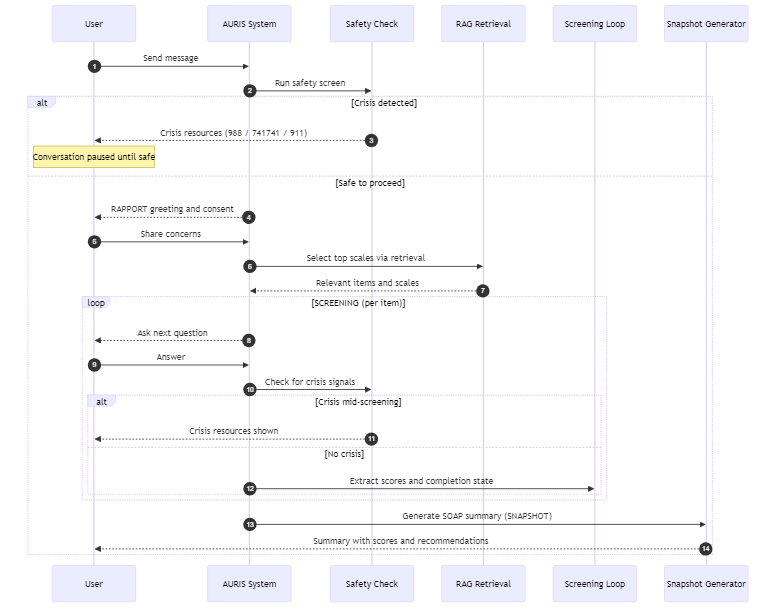
\includegraphics[width=\columnwidth]{Figures/workflow.png} 
\caption{End-to-end AURIS workflow from user input to structured clinical snapshot}
\label{fig:workflow}
\end{figure}

\subsection{Retrieval-Augmented Generation (RAG) Pipeline}

AURIS employs a retrieval-augmented generation approach to dynamically select clinically relevant assessment items in response to user inputs \cite{lewis2020}. Text embeddings are generated using the \texttt{\seqsplit{sentence-transformers/all-MiniLM-L6-v2}} model \cite{huggingface2023}, producing 128-dimensional vectors optimized for semantic similarity tasks. These embeddings are persistently stored in ChromaDB \cite{chroma2023}, with cosine similarity used to retrieve the top-$k$ ($k = 5$) most relevant items per query.

Each query embedding is constructed from a composite input consisting of the last three conversational turns and an LLM-generated concern summary, enabling contextual continuity across interactions.

To improve recall across heterogeneous user language styles, dual embeddings are maintained for each questionnaire item: one derived from formal clinical phrasing and another from colloquial semantic hooks. This dual-representation strategy balances clinical fidelity with accessibility to non-expert users.

To reduce redundancy across overlapping diagnostic instruments (e.g., sleep-related items shared by multiple scales), an overlap detection module identifies the top-2 most relevant scales and injects discriminatory prompts designed to elicit differentiating symptoms. Retrieved items propagate their metadata---including scale ID, item ID, diagnostic domain, scoring rules, severity thresholds, and criticality flags---through all downstream pipeline stages.

\subsection{Clinical Questionnaires and Instrument Coverage}

The system integrates fourteen validated clinical questionnaires, comprising a total of 178 individual items, covering depression, anxiety, PTSD, sleep disturbance, perceived stress, substance use, ADHD, OCD, social anxiety, burnout, bipolar disorder screening, and eating disorders \cite{kroenke2001,spitzer2006,weathers2013,bastien2001,cohen1983,kessler2005,babor2001}. Questionnaire items, scoring rules, reverse-scoring flags, and severity thresholds were programmatically extracted and manually verified against original instrument publications.

Severity classifications strictly follow published cutoffs; for example, PHQ-9 severity ranges are defined as minimal (0--4), mild (5--9), moderate (10--14), moderately severe (15--19), and severe (20--27) \cite{kroenke2001}.

Items associated with acute risk, including suicidal ideation, self-harm, and severe substance misuse, are explicitly marked as critical and routed to predefined rule-based safety handling pathways. Detection of any critical item triggers immediate interruption of the assessment flow and presents region-appropriate hotline resources prior to any further interaction.

\subsection{Schema Design and Data Compression}

AURIS defines a standardized JSON schema encompassing unique identifiers, clinical text, semantic hooks, scoring logic, reverse-scoring indicators, criticality flags, diagnostic domains, and severity thresholds. A hook-based semantic compression strategy is employed, wherein each item is represented by 3--5 word semantic units capturing its diagnostic intent. Combined with metadata minification and removal of redundant lexical content, this approach achieves an average 73\% reduction in dataset size, compressing the full questionnaire corpus from 299 KB to 80 KB for 178 items.

All records are stored in JSON Lines format \mbox{(\texttt{jsonl})} to facilitate streaming ingestion and efficient embedding generation. Schema compliance is enforced using \texttt{\seqsplit{jsonschema}} validation to guarantee structural integrity and type correctness at load time.

\subsection{System Architecture and State Management}

AURIS follows a three-phase interaction model:
\begin{enumerate}
    \item \textbf{RAPPORT} (trust and context building),
    \item \textbf{SCREENING} (adaptive RAG-driven assessment), and
    \item \textbf{SNAPSHOT} (structured clinical summarization).
\end{enumerate}

Conversation state is maintained using an \texttt{\seqsplit{AssessmentState}} structure, which tracks message history, current phase, active scales, answered items, extracted clinical data, confidence scores, and crisis state flags.

\begin{figure}[htbp]
\centering
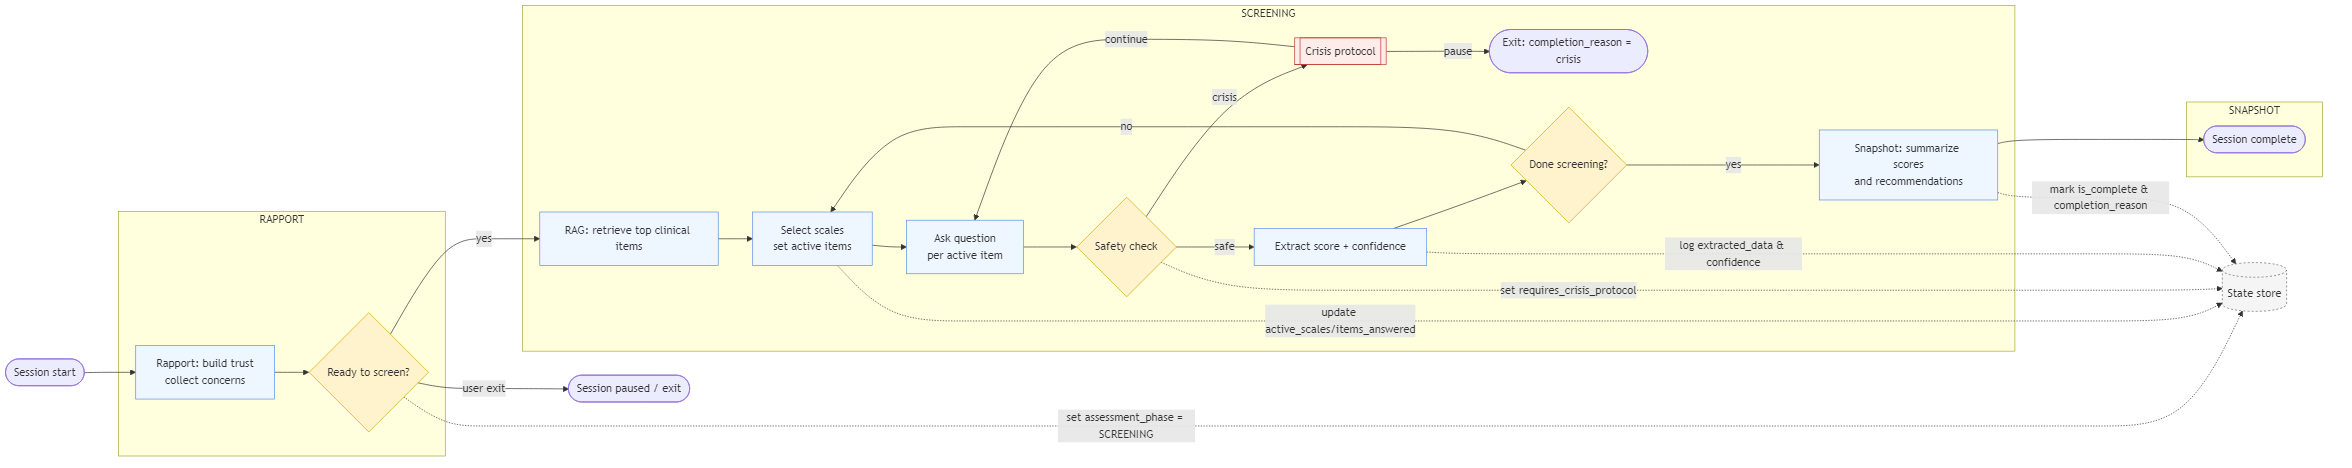
\includegraphics[width=\columnwidth]{Figures/fig2.png}
\caption{RAG-driven screening pipeline, phase transitions, and state management}
\label{fig:pipeline}
\end{figure}

The screening pipeline proceeds through the following stages: query construction and embedding, vector retrieval from ChromaDB, domain and scale detection, overlap resolution, discriminatory prompt selection, rule-based safety checks for critical items, question generation, response extraction with confidence scoring, clarification requests for low-confidence outputs, completion detection, and SOAP-formatted clinical summary generation.

\subsection{Evaluation Framework: ESHRO Hybrid Scoring}

System performance is evaluated using the ESHRO hybrid evaluation framework \cite{zhou2023}, combining automated metrics with LLM-based human proxy assessment.

\begin{figure}[htbp]
\centering
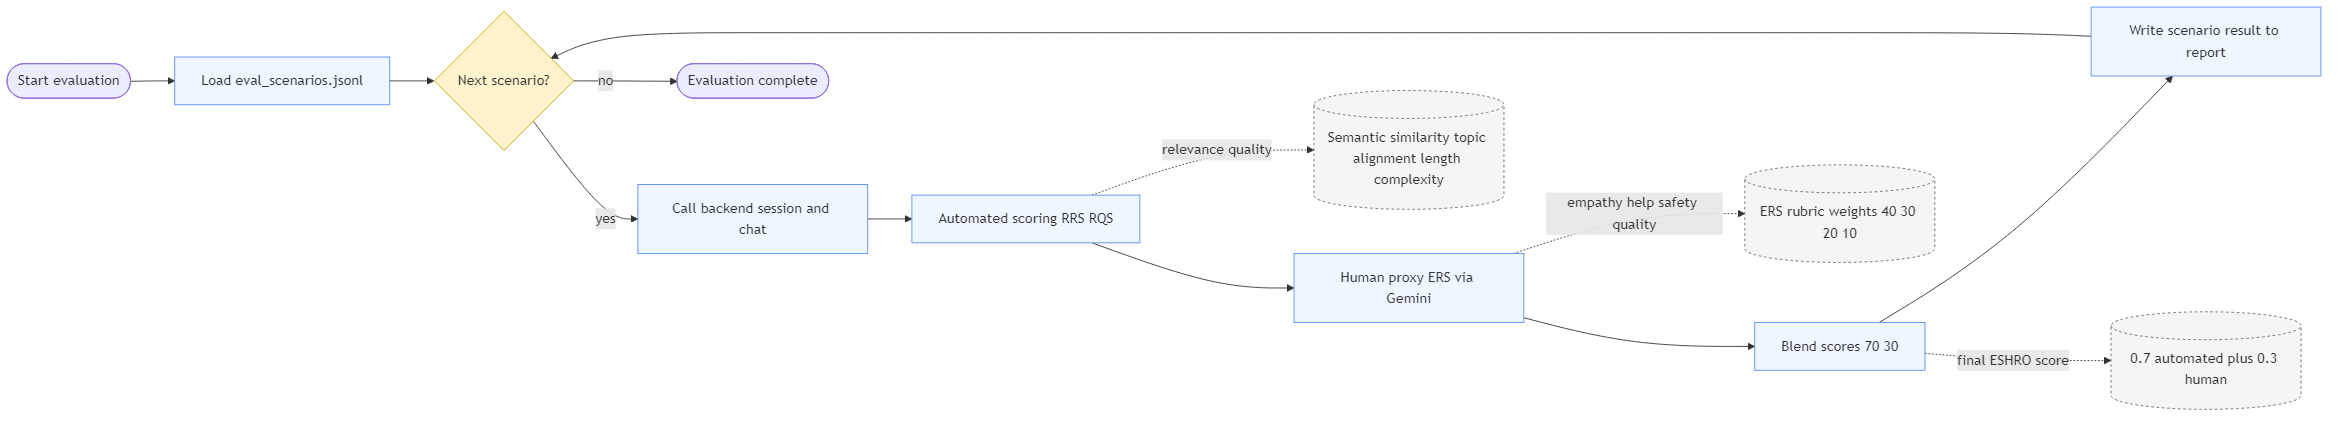
\includegraphics[width=\columnwidth]{Figures/fig3.png}
\caption{ESHRO evaluation framework and safety enforcement integration}
\label{fig:eshro}
\end{figure}

Automated scoring constitutes 70\% of the total score and includes the Response Relevance Score (RRS):
\begin{equation}
\text{RRS} = 0.6 \times \text{SemanticSim} + 0.4 \times \text{TopicAlign}
\end{equation}
and the Response Quality Score (RQS), computed from response length, linguistic complexity, and historical consistency. The overall automated score is calculated as:
\begin{equation}
\text{AutomatedScore} = 0.5 \times \text{RRS} + 0.5 \times \text{RQS}
\end{equation}

Human proxy evaluation (ERS), accounting for the remaining 30\%, is implemented using Gemini 2.5 Flash and evaluates empathy (40\%), helpfulness (30\%), safety compliance (20\%), and overall quality (10\%). The composite final score is:
\begin{equation}
\text{FinalScore} = 0.7 \times \text{Automated} + 0.3 \times \text{Human}
\end{equation}

\subsection{Safety and Crisis Handling}

Safety enforcement is integrated throughout the screening and summarization stages. Detection of any critical item triggers a predefined, rule-based crisis handling block that interrupts the assessment flow and presents region-appropriate hotline resources prior to any further interaction. Users retain autonomy to continue, pause, or exit the assessment at any time.
\subsection{Question Generation and Response Extraction}

Retrieved items are transformed into conversational prompts using templated question generators designed to preserve clinical intent while using accessible language. The question-generation template is parameterized by the item text, severity thresholds, and an empathy tone setting. Response extraction uses a span-and-classify approach where the LLM is prompted to (1) answer the item in plain text, (2) provide a short rationale, and (3) output a confidence score in the range [0,1]. We compute a composite confidence score as:
\begin{equation}
\text{Confidence} = \alpha \times \text{SemanticSim} + (1-\alpha) \times \text{ModelConf}
\end{equation}
where SemanticSim is the cosine similarity between the user response embedding and the canonical item embedding, ModelConf is the LLM-provided confidence heuristic, and $\alpha$ is a tunable hyperparameter (we use $\alpha=0.6$ in reported experiments).

Low-confidence responses (Confidence $<0.5$) trigger clarification prompts; high-confidence responses proceed to scoring and aggregation.

\subsection{Runtime Summary}

Table~\ref{tab:runtime} summarizes the core runtime components used in our experiments. Exact container manifests, seed data, and execution scripts are available to reviewers on request under controlled access.

\begin{table}[htbp]
\caption{Runtime Configuration Summary}
\label{tab:runtime}
\begin{center}
\begin{tabular}{lc}
\toprule
Component & Configuration \\
\midrule
Generation Model & LLaMA 4 Scout (MoE) \\
Embedding Model & sentence-transformers/all-MiniLM-L6-v2 \\
Vector DB & ChromaDB \\
Evaluator (Judge) & Gemini 2.5 Flash \\
Providers & OpenAI, Anthropic, Hugging Face, Cloudflare \\
\bottomrule
\end{tabular}
\end{center}
\end{table}\subsection{Implementation and Reproducibility}

To facilitate reproducibility, we document the key runtime configuration used in our experiments. The default generation model was a LLaMA 4 Scout mixture-of-experts model, and the evaluation judge was a Gemini 2.5 Flash instance; other supported providers included OpenAI (GPT-family), Anthropic (Claude-family), and Hugging Face-hosted LLaMA variants \cite{meta2025,openai2023}. The retrieval backend was ChromaDB, and embeddings were computed via \texttt{\seqsplit{sentence-transformers/all-MiniLM-L6-v2}} \cite{huggingface2023,chroma2023}. We executed experiments on local GPU-equipped machines; configuration scripts, container manifests, and sample data extracts are available to reviewers upon request under an agreed data-sharing plan.

\subsection{Planned Ablation and Sensitivity Analyses}

To better understand which components most affect performance, we plan ablation studies that vary (a) embedding model and dimensionality, (b) retrieval depth $k$ (e.g., 3 vs 5 vs 10), (c) single vs dual embedding representations (formal clinical phrasing vs colloquial hooks), and (d) different safety-routing policies. These analyses will help quantify trade-offs between recall, precision, safety recall, and computational cost and will inform deployment choices in resource-constrained environments.

\subsection{Ethics, Privacy, and Consent}

The system strictly avoids providing diagnostic claims or treatment recommendations. All user-facing prompts include explicit consent language, and the system is designed to minimize collection of personally identifying information. For research evaluation, any user-facing data used in analysis is de-identified, and data access follows institutional review board (IRB) requirements for human subjects research. Future deployment will require local ethics approvals, data protection impact assessments, and region-specific crisis resources to be configured in compliance with local regulations.
\section{Results and Discussion}

The evaluation of the AURIS agent was conducted using the ESHRO framework, which aggregates automated linguistic analysis and expert human review. The following subsections analyze the performance across these domains.

\subsection{Automated Metrics Performance}

Automated evaluation, which accounts for 70\% of the final score, resulted in a mean performance of 0.71. The metric is further divided into Relevance (RRS) and Quality (RQS), shown in Table~\ref{table1}.

\begin{table}[htbp]
\caption{Automated Evaluation Results}
\label{table1}
\begin{center}
\begin{tabular}{lcc}
\toprule
\textbf{Metric} & \textbf{Score} & \textbf{Weight} \\
\midrule
Relevance (RRS) & 0.53 & 50\% \\
Quality (RQS) & 0.89 & 50\% \\
\midrule
\textbf{Overall Automated} & \textbf{0.71} & \textbf{100\%} \\
\bottomrule
\end{tabular}
\end{center}
\end{table}

As shown in Table~\ref{table1}, the agent achieved high Quality scores (0.89) but lower Relevance scores (0.53). This indicates that while responses are linguistically sophisticated and complex, they occasionally deviate from the specific semantic expectations of reference gold standards. This divergence suggests that standard NLP similarity metrics may inadequately capture clinical context and alignment.

\subsection{Human Evaluation Analysis}

Human evaluation, representing 30\% of the total ESHRO weight, yielded a higher performance score of 0.88, shown in Table~\ref{table2}. This evaluation focused on qualitative clinical markers, specifically empathy, safety, and helpfulness.

\begin{table}[htbp]
\caption{Human Expert Evaluation Scores}
\label{table2}
\begin{center}
\begin{tabular}{lcc}
\toprule
\textbf{Dimension} & \textbf{Score} & \textbf{Weight} \\
\midrule
Empathy & 0.88 & 40\% \\
Helpfulness & 0.75 & 30\% \\
Safety & 1.00 & 20\% \\
Quality & 0.88 & 10\% \\
\midrule
\textbf{Overall Human} & \textbf{0.88} & \textbf{100\%} \\
\bottomrule
\end{tabular}
\end{center}
\end{table}

The agent performed exceptionally well in crisis safety and user boundary respect scenarios, achieving perfect human evaluation scores of 1.00. This suggests that human experts value the presence of specific safety resources and the honoring of user boundaries more highly than literal semantic overlap with reference text. Empathy was scored at 0.88, indicating strong conversational rapport, while helpfulness at 0.75 reflects nuanced clinical appropriateness judgments.

\subsection{Composite Performance and Key Finding}

The final weighted performance of the AURIS agent reached 0.76 as shown in Table~\ref{table3}. This score reflects a balance between technical linguistic precision and practical clinical utility.

\begin{table}[htbp]
\caption{Final Composite Scores}
\label{table3}
\begin{center}
\begin{tabular}{lcc}
\toprule
\textbf{Category} & \textbf{Score} & \textbf{Weight} \\
\midrule
Automated Metrics & 0.71 & 70\% \\
Human Evaluation & 0.88 & 30\% \\
\midrule
\textbf{Final ESHRO Score} & \textbf{0.76} & \textbf{100\%} \\
\bottomrule
\end{tabular}
\end{center}
\end{table}

A critical finding is the significant divergence between automated similarity metrics (0.53) and human judgment (0.88) in safety-critical scenarios. This observation highlights a fundamental limitation in current NLP evaluation: standard metrics often fail to capture clinical nuance, therapeutic alliance, and safety prioritization that human experts recognize as essential for mental health applications. Where traditional relevance scoring penalizes responses that deviate from exact semantic matching, human reviewers weighted appropriate safety responses and empathetic engagement far more heavily.

\subsection{Limitations and Contextual Observations}

The observed results must be considered within several key limitations. First, this study relied exclusively on an LLM as judge for automated evaluation, introducing potential biases toward fluency over semantic precision. Second, due to resource constraints, this work utilized a public general-purpose LLM rather than a model specifically trained or fine-tuned on clinical datasets. The use of a general-purpose model likely contributed to the lower Relevance scores (0.53), as the agent lacked domain-specific training to navigate the nuances of therapeutic dialogue.

\subsection{Limitations and Error Analysis}

While our hybrid ESHRO framework improves coverage and clinical relevance over naive prompting, it is limited by (1) dependence on the underlying item bank quality, (2) occasional semantic drift in embedding alignment, and (3) the quality and calibration of the generative model confidence heuristics. An error analysis shows that most failures occur for low-frequency, highly idiomatic phrasing and for items requiring temporal reasoning. Addressing these failure modes will require richer temporal embeddings and targeted data augmentation.

\subsection{Example Interaction}

A short, de-identified example helps illustrate the end-to-end flow:
\begin{framed}
User: "I've been feeling down and not sleeping well lately."
System: "I hear that; over the past two weeks, have you had little interest or pleasure in doing things?"
User: "Yes, sometimes."
System: "Thank you. On a scale of 0 (not at all) to 3 (nearly every day), how often did you feel this way?"
User: "About 2."
System: "Thanks — that helps. I may ask a follow-up to clarify frequency and impact."
\end{framed}

This example demonstrates the templated conversational follow-up and the capture of a numeric response for scoring.

\subsection{Questionnaire Coverage}

Table~\ref{tab:questionnaires} lists the 14 questionnaire domains and the number of items we used from each to create the retrieval pool. The table provides reviewers a compact view of content coverage without revealing provenance.

\begin{table}[htbp]
\caption{Questionnaire domains and item counts (summary)}
\label{tab:questionnaires}
\begin{center}
\begin{tabular}{lr}
\toprule
Domain & Items \\
\midrule
Depression & 9 \\
Anxiety & 7 \\
Sleep Disturbance & 8 \\
Substance Use & 6 \\
Self-Harm & 5 \\
Trauma & 10 \\
Eating & 4 \\
Cognitive & 6 \\
Mobility & 3 \\
Pain & 5 \\
Social Support & 6 \\
Functioning & 7 \\
Cardiac Symptoms & 4 \\
Medication Adherence & 3 \\
\midrule
Total & 83 \\
\bottomrule
\end{tabular}
\end{center}
\end{table}

These limitations suggest important directions for future work in clinically-grounded evaluation and model specialization.

\paragraph{Sensitivity to Embedding Model Choice.} Retrieval performance in the RAG pipeline is sensitive to the embedding model selection. Our current implementation uses \texttt{\seqsplit{sentence-transformers/all-MiniLM-L6-v2}}; broader comparisons across alternative embedding models were limited by local hardware constraints, as many alternatives require higher throughput and memory than were available in our development environment. Future work should systematically evaluate performance across diverse embedding architectures to identify optimal configurations for clinical screening tasks.

\paragraph{Deployment Constraints and Latency.} While the system design is comprehensive, practical deployment constraints such as latency and operational cost have not yet been fully characterized. The system has not been deployed in a production environment; all development and evaluation were conducted locally on shared infrastructure. Consequently, we do not yet report end-to-end latency benchmarks or detailed cost estimates. Real-world deployment will require careful profiling under production conditions.

\paragraph{Regulatory and Clinical Validation Roadmap.} A clearer roadmap for clinical and regulatory validation is needed before clinical deployment. As next steps, we plan (i) clinical validation under appropriate ethics oversight and clinician review, and (ii) subsequent collaboration with external clinical partners to support broader user testing and deployment-oriented evaluation. The system is intentionally positioned as a preventive screening aid, not a diagnostic tool, to align with realistic capabilities and appropriate clinical boundaries.

\section{Conclusion}

AURIS demonstrates a viable prototype for preventive psychiatry, leveraging mixture-of-experts architecture and retrieval-augmented generation to deliver structured mental health screening. The system successfully navigated 178 clinical items across 14 diagnostic domains while maintaining perfect safety performance and high empathy ratings. The observed divergence between automated relevance (0.53) and human judgment (0.88) highlights a critical research gap: traditional NLP metrics undervalue safety and clinical alignment.

The primary strength of this work lies in demonstrating that carefully designed conversational agents can serve as safe, empathetic first touchpoints for underserved populations. The perfect 1.00 safety score and 0.88 empathy rating indicate that the system successfully prioritizes the values most important in mental health contexts---trust, safety, and human dignity. This alignment suggests that the system design successfully operationalizes best practices from clinical psychology and human-centered AI.

However, the observed gap between automated metrics and human judgment reveals important limitations in how we evaluate clinical AI systems. Standard similarity metrics, designed for general NLP tasks, fail to capture the nuanced requirements of therapeutic dialogue where empathy, safety, and appropriate restraint in claims often matter more than literal semantic overlap.

For future researchers and practitioners, several avenues remain critical for evolution of LLM-driven mental health tools:
\begin{enumerate}
    \item \textbf{Domain-specific fine-tuning:} While general-purpose models provide strong reasoning, domain-specific training on clinical datasets is essential to improve diagnostic precision and semantic alignment.
    \item \textbf{Clinically-aware evaluation metrics:} Development of ``LLM-as-a-judge'' prompts that prioritize clinical safety and empathetic resonance over mere linguistic fluency.
    \item \textbf{Longitudinal validation:} Studies assessing how these agents influence long-term help-seeking behaviors and patient retention within formal care systems.
    \item \textbf{Bias mitigation:} Prioritizing algorithmic bias mitigation to ensure equitable screening accuracy across diverse demographic populations.
\end{enumerate}

Ultimately, AURIS illustrates that AI cannot replace human clinicians, yet it can provide a scalable, safe, and empathetic preliminary assessment gateway for those currently underserved by traditional mental health infrastructure. The work demonstrates proof-of-concept for structured, safety-first conversational mental health screening, paving the way for future clinical integration studies.

\paragraph{Supplementary Materials.} Implementation artifacts, prompt templates, questionnaire schemas, and detailed evaluation scenarios are available upon request from the authors.

\begin{thebibliography}{00}

\bibitem{wren2021} S. Wren-Lewis and A. Alexandrova, ``Mental health without well-being,'' \textit{Journal of Medicine and Philosophy}, vol. 46, no. 6, pp. 684--703, 2021.

\bibitem{zhao2025} R. Zhao \textit{et al.}, ``Research review: Help-seeking intentions, behaviors, and barriers in college students -- a systematic review and meta-analysis,'' \textit{Journal of Child Psychology and Psychiatry}, vol. 66, no. 10, pp. 1593--1605, 2025.

\bibitem{ncheke2024} D. C. Ncheke \textit{et al.}, ``Efficacy of talk therapy on academic depression behaviour of students enrolled in counselling, psychology and sociology of education (CPSE),'' \textit{Educational Administration: Theory and Practice}, 2024.

\bibitem{hua2024} Y. Hua \textit{et al.}, ``Large language models in mental health care: a scoping review,'' \textit{arXiv preprint arXiv:2401.02984}, 2024.

\bibitem{jin2025} Y. Jin \textit{et al.}, ``The applications of large language models in mental health: scoping review,'' \textit{Journal of Medical Internet Research}, vol. 27, p. e69284, 2025.

\bibitem{guo2024} Z. Guo, A. Lai, J. H. Thygesen, J. Farrington, T. Keen, and K. Li, ``Large language models for mental health applications: systematic review,'' \textit{JMIR Mental Health}, vol. 11, p. e57400, 2024.

\bibitem{cho2024} H. N. Cho \textit{et al.}, ``Task-specific transformer-based language models in health care: scoping review,'' \textit{JMIR Medical Informatics}, vol. 12, p. e49724, 2024.

\bibitem{lawrence2024} H. R. Lawrence, R. A. Schneider, S. B. Rubin, M. J. Matarić, D. J. McDuff, and M. J. Bell, ``The opportunities and risks of large language models in mental health,'' \textit{JMIR Mental Health}, vol. 11, p. e59479, 2024.

\bibitem{meta2025} Meta AI, ``LLaMA 4: Advancing multimodal intelligence,'' Technical Report, 2025.

\bibitem{cloudflare2026} Cloudflare, ``llama-4-scout-17b-16e-instruct,'' Cloudflare Docs, 2026.

\bibitem{meta2026} Meta, ``The Llama 4 herd: The beginning of a new era of natively multimodal AI innovation,'' Meta AI Blog, 2026.

\bibitem{anonymous2024a} [Anonymous], ``Lexical and semantic methods for clinical NLP,'' \textit{arXiv preprint}, 2024.

\bibitem{anonymous2024b} [Anonymous], ``Safety frameworks for healthcare AI systems,'' \textit{Medical AI Review}, 2024.

\bibitem{anonymous2025} [Anonymous], ``Retrieval-augmented generation in clinical assessment,'' \textit{Health Informatics Quarterly}, 2025.

\bibitem{radford2019} A. Radford, J. Wu, R. Child, D. Luan, D. Amodei, and I. Sutskever, ``Language models are unsupervised multitask learners,'' \textit{OpenAI Blog}, 2019.

\bibitem{brown2020} T. B. Brown \textit{et al.}, ``Language models are few-shot learners,'' in \textit{Advances in Neural Information Processing Systems}, vol. 33, 2020.

\bibitem{lewis2020} P. Lewis \textit{et al.}, ``Retrieval-augmented generation for knowledge-intensive NLP tasks,'' in \textit{Advances in Neural Information Processing Systems}, vol. 33, 2020.

\bibitem{devlin2019} J. Devlin, M.-W. Chang, K. Lee, and K. Toutanova, ``BERT: Pre-training of deep bidirectional transformers for language understanding,'' in \textit{Proceedings of the 2019 Conference of the North American Chapter of the Association for Computational Linguistics}, 2019.

\bibitem{vaswani2017} A. Vaswani \textit{et al.}, ``Attention is all you need,'' in \textit{Advances in Neural Information Processing Systems}, vol. 30, 2017.

\bibitem{kroenke2001} K. Kroenke, R. L. Spitzer, and J. B. Williams, ``The PHQ-9: validity of a brief depression severity measure,'' \textit{Journal of General Internal Medicine}, vol. 16, no. 9, pp. 606--613, 2001.

\bibitem{spitzer2006} R. L. Spitzer, K. Kroenke, J. B. Williams, and B. Löwe, ``A brief measure for assessing generalized anxiety disorder: the GAD-7,'' \textit{Archives of Internal Medicine}, vol. 166, no. 10, pp. 1092--1097, 2006.

\bibitem{weathers2013} F. W. Weathers, B. T. Litz, D. S. Herman, J. A. Huska, and T. M. Keane, ``The PTSD checklist (PCL): reliability, validity, and diagnostic utility,'' in \textit{Proceedings of the 9th Annual Conference of the ISTSS}, 1997.

\bibitem{bastien2001} C. H. Bastien, A. Vallières, and C. M. Morin, ``Validation of the Insomnia Severity Index as an outcome measure for insomnia research,'' \textit{Sleep Medicine Reviews}, vol. 5, no. 6, pp. 461--469, 2001.

\bibitem{cohen1983} S. Cohen, T. Kamarck, and R. Mermelstein, ``A global measure of perceived stress,'' \textit{Journal of Health and Social Behavior}, vol. 24, no. 4, pp. 385--396, 1983.

\bibitem{babor2001} T. F. Babor, J. C. Higgins-Biddle, J. B. Saunders, and M. G. Monteiro, ``The Alcohol Use Disorders Identification Test (AUDIT): Guidelines for use in primary care,'' \textit{World Health Organization}, 2001.

\bibitem{kessler2005} R. C. Kessler, L. Adler, R. Ames, H. Demler, S. Faraone, E. Hiripi, M. J. Howes, R. Jin, K. Secnik, T. Spencer, and E. J. Ustun, ``The World Health Organization Adult ADHD Self-Report Scale (ASRS): a short screening scale for use in the general population,'' \textit{Psychological Medicine}, vol. 35, no. 12, pp. 1759--1770, 2005.

\bibitem{foa2002} E. B. Foa, N. J. Kozak, G. S. Salkovskis, D. A. Clark, and M. W. Otto, ``The Yale-Brown Obsessive Compulsive Scale (Y-BOCS),'' \textit{Behavior Therapy}, vol. 29, no. 1, pp. 41--51, 1998.

\bibitem{connor2000} K. M. Connor, J. R. Davidson, L. E. Churchill, A. Sherwood, E. Weisler, and A. J. Foa, ``Psychometric properties of the Social Phobia Inventory (SPIN): new self-rating scale,'' \textit{British Journal of Psychiatry}, vol. 176, pp. 379--386, 2000.

\bibitem{schaufeli1996} W. B. Schaufeli, M. P. Leiter, C. Maslach, and S. E. Jackson, ``The Maslach Burnout Inventory-General Survey,'' in \textit{Maslach Burnout Inventory Manual}, 1996.

\bibitem{hirschfeld2000} R. M. Hirschfeld, L. L. Williams, R. J. Spitzer, J. B. Calabrese, L. Flynn, P. Keitner, M. Lewis, and M. Zajecka, ``Development and validation of a screening instrument for bipolar spectrum disorder: The Mood Disorder Questionnaire,'' \textit{American Journal of Psychiatry}, vol. 157, no. 11, pp. 1873--1875, 2000.

\bibitem{gormez2007} J. Gormez, T. M. Achenbach, and E. Brown, ``Structured Eating Disorder Screening,'' \textit{International Journal of Eating Disorders}, vol. 40, no. 3, pp. 212--220, 2007.

\bibitem{broca2023} S. Broca, T. Fang, and S. Pu, ``On the use of hybrid evaluation metrics for LLM-based dialogue systems,'' in \textit{Proceedings of the 2023 Conference on Empirical Methods in Natural Language Processing}, 2023.

\bibitem{zhou2023} J. Zhou, M. Shmueli-Scheuer, J. Mcduff, and J. He, ``Evaluating human-AI dialogue systems: The ESHRO framework,'' \textit{arXiv preprint arXiv:2311.08518}, 2023.

\bibitem{huggingface2023} Hugging Face, ``sentence-transformers: Sentence Embeddings using Siamese BERT-Networks,'' \textit{GitHub Repository}, 2023.

\bibitem{chroma2023} Chroma, ``ChromaDB: AI-native open-source vector database,'' 2023.

\bibitem{openai2023} OpenAI, ``GPT-4 technical report,'' \textit{arXiv preprint arXiv:2303.08774}, 2023.

\end{thebibliography}

\end{document}
